%%%%%%%%%%%%%%%%%%%%%%%%%%%%%%%%%%%%%%%%%%%%%%%%%%%%%%%%%%%%%%%%%
% MUW Presentation
% LaTeX Template
% Version 1.0 (27/12/2016)
%
% License:
% CC BY-NC-SA 4.0 (http://creativecommons.org/licenses/by-nc-sa/3.0/)
%
% Created by:
% Nicolas Ballarini, CeMSIIS, Medical University of Vienna
% nicoballarini@gmail.com
% http://statistics.msi.meduniwien.ac.at/
%
% Customized for UAH by:
% David F. Barrero, Departamento de Automática, UAH
%%%%%%%%%%%%%%%%%%%%%%%%%%%%%%%%%%%%%%%%%%%%%%%%%%%%%%%%%%%%%%%%%

\documentclass[10pt,compress]{beamer} % Change 10pt to make fonts of a different size
\mode<presentation>

\usepackage[spanish]{babel}
\usepackage{fontspec}
\usepackage{tikz}
\usepackage{etoolbox}
\usepackage{xcolor}
\usepackage{xstring}
\usepackage{listings}
\usepackage{tikz}
\usetikzlibrary{matrix,chains,positioning,decorations.pathreplacing,arrows,shapes}

\usetheme{UAH}
\usecolortheme{UAH}
\setbeamertemplate{navigation symbols}{} 
\setbeamertemplate{caption}[numbered]

%%%%%%%%%%%%%%%%%%%%%%%%%%%%%%%%%%%%%%%%%%%%%%%%%%%%%%%%%%%%%%%%%
%% Presentation Info
\title[Modules]{Modules}
\author{}
\institute{\asignatura}
\date{}
%%%%%%%%%%%%%%%%%%%%%%%%%%%%%%%%%%%%%%%%%%%%%%%%%%%%%%%%%%%%%%%%%


%%%%%%%%%%%%%%%%%%%%%%%%%%%%%%%%%%%%%%%%%%%%%%%%%%%%%%%%%%%%%%%%%
%% Descomentar para habilitar barra de navegación superior
\ponerNavegacion
%%%%%%%%%%%%%%%%%%%%%%%%%%%%%%%%%%%%%%%%%%%%%%%%%%%%%%%%%%%%%%%%%

%%%%%%%%%%%%%%%%%%%%%%%%%%%%%%%%%%%%%%%%%%%%%%%%%%%%%%%%%%%%%%%%%
%% Configuración de logotipos en portada
%% Opacidad de los logotipos
\newcommand{\opacidad}{1}
%% Descomentar para habilitar logotipo en pié de página de portada
\renewcommand{\logoUno}{Images/isg.png}
%% Descomentar para habilitar logotipo en pié de página de portada
%\renewcommand{\logoDos}{Images/CCLogo.png}
%% Descomentar para habilitar logotipo en pié de página de portada
%\renewcommand{\logoTres}{Images/ALogo.png}
%% Descomentar para habilitar logotipo en pié de página de portada
%\renewcommand{\logoCuatro}{Images/ELogo.png}
%%%%%%%%%%%%%%%%%%%%%%%%%%%%%%%%%%%%%%%%%%%%%%%%%%%%%%%%%%%%%%%%%

%%%%%%%%%%%%%%%%%%%%%%%%%%%%%%%%%%%%%%%%%%%%%%%%%%%%%%%%%%%%%%%%%
%% FOOTLINE
%% Comment/Uncomment the following blocks to modify the footline
%% content in the body slides. 


%% Option A: Title and institute
\footlineA
%% Option B: Author and institute
%\footlineB
%% Option C: Title, Author and institute
%\footlineC
%%%%%%%%%%%%%%%%%%%%%%%%%%%%%%%%%%%%%%%%%%%%%%%%%%%%%%%%%%%%%%%%%

\begin{document}

%%%%%%%%%%%%%%%%%%%%%%%%%%%%%%%%%%%%%%%%%%%%%%%%%%%%%%%%%%%%%%%%%
% Use this block for a blue title slide with modified footline
{\titlepageBlue
    \setbeamertemplate{headline}{}
	\setbeamercolor{frametitle}{bg=black}
	\setbeamercolor{normal text}{bg=black}
    \begin{frame}
        \titlepage
    \end{frame}
}

\begin{frame}[plain]{}
	\begin{block}{Objectives}
		\begin{enumerate}
		\item Understand the relevance to use modules and packages.
		\item Be able to install some widely used Python packages about  geospatial software.
		\item Be able to apply some modules and packages of both Python Standard Library and others Python Geospatial Libraries.
		\end{enumerate}
	\end{block}
\end{frame}

{
\eliminarNavegacion
\begin{frame}[shrink]{Table of Contents}
 \frametitle{Table of Contents}
 \tableofcontents
  % You might wish to add the option [pausesections]
\end{frame}
}

\section{Introduction}
\begin{frame}{Introduction (I)}
		You loose everything when exit the interpreter
			\begin{itemize}
			\item \textit{Solution}: Write it down in a script
			\end{itemize}
		When a script becomes big, it is difficult to maintain
			\begin{itemize}
			\item \textit{Solution}: Split your script in several ones
			\end{itemize}
		As you get more scripts, you will need to reuse your functions
			\begin{itemize}
			\item \textit{Solution}: Create a \alert{module}
			\item \textbf{Module}: A file that contains definitions, functions and classes
			\end{itemize}
		If a module is too big, it is too difficult to maintain
			\begin{itemize}
			\item \textit{Solution}: Create a \alert{package}
			\item \textbf{Package}: A module of modules
			\end{itemize}
\end{frame}

\begin{frame}{Introduction (II)}
		\begin{block}{Why modules?}
			\begin{itemize}
			\item \textbf{Main function}: Organization.
			\item \textbf{Reuse}: To provide software solutions, that have been proven to work, to solve similar problems.
			\end{itemize}
		\end{block}
		
\end{frame}

\section{Modules}

\subsection{Using modules}
\begin{frame}{Using modules}{Creation and Implementation}
	\vspace{-0.2cm}
	A module is just a Python script with \texttt{.py} extension
	\vspace{-0.2cm}
	%creo que está mal fibo.py
	\begin{block}{fibo.py}
	\vspace{-0.2cm}
	\lstinputlisting[basicstyle=\scriptsize,numbers=left]{code/fibo.py}
	\vspace{-0.2cm}
	\end{block}
\end{frame}

\begin{frame}{Using modules}{Where is it stored?}

 Accessible and reusable module:
 \begin{itemize}
 \item  Set path in the file directory where the module is stored.
 \item Variable \texttt{PYTHONPATH}
 \end{itemize}
 \end{frame}
 
\begin{frame}[fragile]{Using modules}{How do I use them? (I)}
	\begin{block}{}
	\begin{verbatim}
	>>> import fibo
	>>> fibo.fib(1000)
	1 1 2 3 5 8 13 21 34 55 89 144 233 377 610 987
	>>> fibo.fib2(100)
	[1, 1, 2, 3, 5, 8, 13, 21, 34, 55, 89]
	>>> fibo.__name__
	'fibo'
	>>> fib = fibo.fib
	>>> fib(100)
	1 1 2 3 5 13 21 34 55 89
	\end{verbatim}
	\vspace{-0.2cm}
	\end{block}
\end{frame}

\begin{frame}[fragile]{Using modules}{How do I use them?  (II)}
	A module can import other modules
		\begin{itemize}
		\item Name conflicts may arise: Each module has a symbol table
		\item It means you should invoke it as \texttt{modname.itemname}
		\end{itemize}
 	It is possible to import items directly
		\begin{itemize}
		\item \texttt{from module import name1, name2}
		\item \texttt{from module import *}
		\item It uses the global symbol table (no need to use the modname)
			\end{itemize}
	
	\begin{block}{}
	\begin{verbatim}
	>>> from fibo import fib, fib2
	>>> fib(100)
	1 1 2 3 5 8 13 21 34 55 89 144 233 377 610 987
	\end{verbatim}
	\end{block}
\end{frame}

\begin{frame}[fragile]{Using modules}{How do I use them?  (III)}
	\vspace{-0.2cm}
	\begin{block}{List zip file contents (file.zip must exist. Open in read mode)}
	\vspace{-0.2cm}
	\lstinputlisting[numbers=left]{code/zip.py}
	\vspace{-0.2cm}
	\end{block}
	
	\vspace{-0.2cm}
	\centering \footnotesize{Several examples here: \url{http://pymotw.com/2/PyMOTW-1.132.pdf}}
\end{frame}

\begin{frame}[fragile]{Using modules}{How do I use them?  (IV)}
	%\vspace{-0.2cm}
	Error while importing:
	\begin{itemize}
	\item The module does not exist.
	\item The module name has not been well written.
	\item The module is not on the search path of Python modules:
	\begin{enumerate}
	\item By default, it searches in the current directory.
	\item If it does not find it here, it then searches in the directories of the environment variable \texttt{PYTHONPATH}.
	\begin{itemize}
	\item \texttt{echo \$PYTHONPATH}
	\item \texttt{import sys}\\
	\texttt{print sys.path}
	\end{itemize}
	\item If it still does not find, it then searches in the installation directories of Python.
	\end{enumerate}
	\item How can I troubleshoot it?
	\end{itemize}
\end{frame} 
	
\subsection{Executing modules}

\begin{frame}{Executing modules}{Modules as scripts (I)}
	When a module is imported, its statements are executed
		\begin{itemize}
		\item It declares functions, classes, variables ...
		\item ... and also executes code
		\item It serves to initialize the module
		\end{itemize}
	Very useful to use modules as programs and libraries
\end{frame}

\begin{frame}[shrink,plain,fragile]{Executing modules}{Modules as scripts (II)}
	\vspace{-0.3cm}
	\begin{block}{fibo2.py}
	\vspace{-0.2cm}
	\lstinputlisting[numbers=left]{code/fibo2.py}
	\vspace{-0.2cm}
	\end{block}

	\begin{block}{}
	\vspace{-0.2cm}
	\begin{verbatim}
    (python3 version)	
	$ python3 fibo2.py 50
	1 1 2 3 5 8 13 21 34
	\end{verbatim}
	\vspace{-0.2cm}
	\end{block}
\end{frame}

\subsection{Compiled Python files}
\begin{frame}{Compiled Python files}{}
	We said Python is an interpreted language
		\begin{itemize}
		\item ... this is almost a lie
		\end{itemize}
	Python, as other interpreted languages, has a speed-up trick
		\begin{itemize}
		\item It can use bytecode, just as Java
		\end{itemize}
	\textbf{Bytecode}: Intermediate code between machine code and source code
		\begin{itemize}
		\item Faster than source code, slower than machine code.
		\item It is transparent to the programmer.
		\item The first time a \texttt{.py} file is executed, it is compiled automatically, generating a \texttt{.pyc} file.
		\end{itemize}
\end{frame}

\subsection{Content of a module}

\begin{frame}[fragile]{Content of a module}{The dir() function}
	Very usefull to get an insight to a module
	\begin{itemize}
		\item It returns the names defined in a module
		\item Without arguments, it returns your names
	\end{itemize}
	\begin{block}{}
	\begin{verbatim}
	>>> import fibo, sys
	>>> dir(fibo)
	['__name__', 'fib', 'fib2']
	>>> dir()
	['__builtins__', ... , '__spec__']
	>>> variable = 'Hello'
	>>> dir()
	['__builtins__', ... , '__spec__', 'variable']
	\end{verbatim}
	\vspace{-0.2cm}
	\end{block}
\end{frame}

\section{Packages}
\subsection{Package concept}
\begin{frame}{Packages}{Package concept (I)}
		If a module gets too big, many problems arise
			\begin{itemize}
			\item Name collisions
			\item It is good to organize modules in a bigger structure: \textit{Packages}
			\end{itemize}
		Packages can be seen as ``dotted module names''
			\begin{itemize}
			\item It is just a module that contains more modules
			\item Make life easier in big proyects
			\item The name \texttt{A.B} designates a submodule \texttt{B} in a package named \texttt{A}
			\end{itemize}
		Must contain a \texttt{\_\_init\_\_.py} file in the root directory
			\begin{itemize}
			\item Executed when the package is imported for the first time
			\end{itemize}
\end{frame}

\begin{frame}[shrink,plain]{Packages}{Package concept (II)}
	\centering \textit{Sound module structure}
	\lstinputlisting{code/module.txt}
\end{frame}

\subsection{Importing a package}
\begin{frame}{Packages}{Importing a package (I)}
	\centering{\alert{Ways to use a package}}\\
	\bigskip
	\begin{flushleft}
	Import an individual module
		\begin{itemize}
		\item \texttt{import sound.effects.echo}
		\item Use function as \texttt{sound.effects.echo.echofilter(input, output)}
		\end{itemize}
	Alternative way to import an individual module
		\begin{itemize}
		\item \texttt{from sound.effects import echo}
		\item Use function as \texttt{echo.echofilter(input, output)}
		\end{itemize}
	Alternative way to import an individual module
		\begin{itemize}
		\item \texttt{from sound.effects.echo import echofilter}
		\item Use function as \texttt{echofilter(input, output)}
		\end{itemize}
	\end{flushleft}
\end{frame}

\begin{frame}{Packages}{Importing a package (II)}
	Imagine we run \texttt{from sound import *}
		\begin{itemize}
		\item In theory, it would import the whole package
		\item In practice, it would take too much time
		\end{itemize}
	There is a convention to avoid waste of resources
		\begin{itemize}
		\item There may be a variable \texttt{\_\_all\_\_} defined in \texttt{\_\_init\_\_}
		\item \texttt{\_\_all\_\_} contains modules to be imported
		\end{itemize}

	\begin{block}{sounds/effects/\_\_init\_\_.py}
	\vspace{-0.2cm}
	\lstinputlisting{code/package.py}
	\vspace{-0.2cm}
	\end{block}
\end{frame}

\subsection{Installing packages}
\begin{frame}[fragile]{Packages}{Installing packages}
	Command-line automatic tool:\texttt{pip} 
		\begin{itemize}
			\item Very similar to \texttt{apt-get} in Linux
		\end{itemize}

	\begin{block}{pip usage}
	\begin{verbatim}
		$ python -m pip install SomePackage
	\end{verbatim}
	\end{block}

	\begin{block}{pip alternative usage}
	\begin{verbatim}
		$ pip3 install SomePackage
	\end{verbatim}
	\end{block}
	Example of the PIL  installation:\\
	\texttt{\$ pip3 install Pillow}\\
\alert{\href{http://recursospython.com/guias-y-manuales/instalacion-y-utilizacion-de-pip-en-windows-linux-y-os-x/}{(More info)}}
\end{frame}

\subsection{What has been developed about Python packages?}
\begin{frame}{Packages}{What has been developed?}
\centering 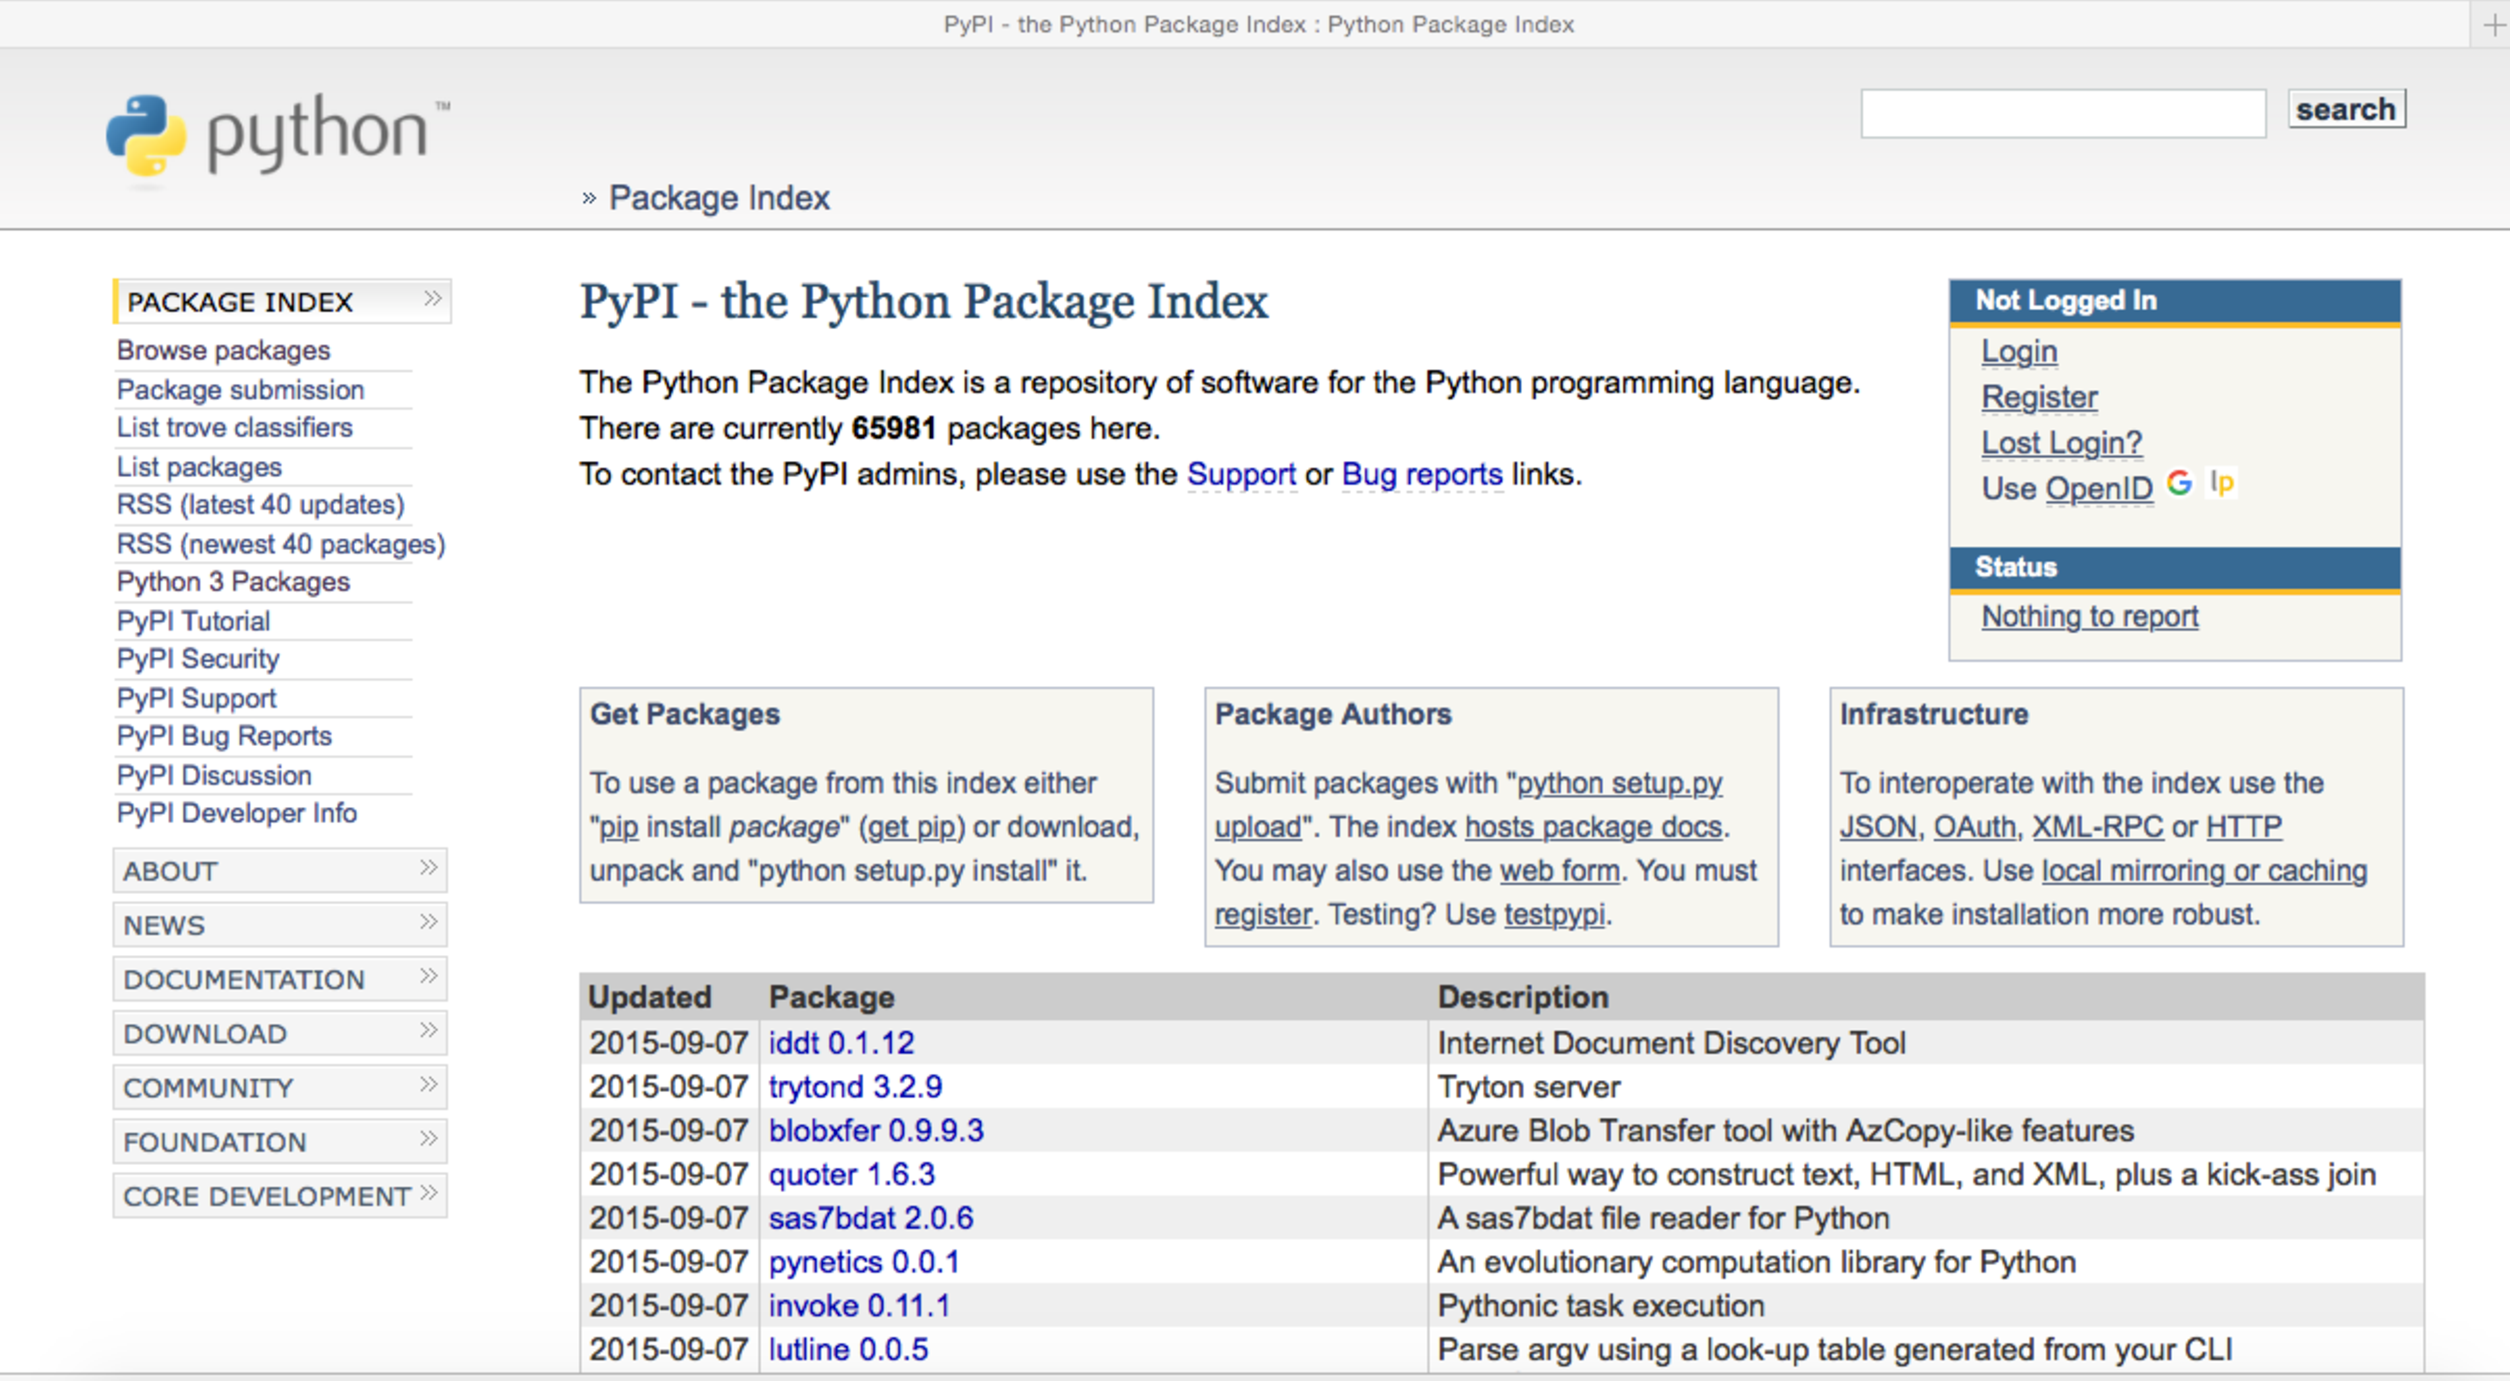
\includegraphics[scale=0.267]{figs/PyPI.pdf}\\
\end{frame}


\section{The Python Standard Library}

\subsection{\texttt{os} module}

\begin{frame}{\texttt{os} module}{Functions to manipulate files and processes}
\vspace{-0.2cm}
\footnotesize{
\begin{block}{}
\vspace{-0.15cm}

\begin{itemize}			
\item \textbf{Functions for managing files and paths}: \texttt{os.path}
\item \textbf{Create directories}. Example: \texttt{os.mkdir('data')}
\item \textbf{Current working directory}: \texttt{os.getcwd()}
\item \textbf{Moving to a certaing directory}. Example: \texttt{os.chdir('data')}
\item \textbf{Value of an environment variable}. Example: \texttt{os.chdir(os.environ['HOME'])}
\item \textbf{Rename a file}. Example: \texttt{os.rename('fich1.py', 'palindrome.py')}
\item \textbf{Deleting a file}. Example: \texttt{os.remove('practica1.py')}
\item \textbf{List the files in the current directory}. Example: \texttt{os.listdir(os.curdir)}
\item \textbf{List the files in a certain directory}. Example: \texttt{os.listdir('c:$\backslash\backslash$data')}
\item \textbf{Call operating system (execute OS services)}. Example: \texttt{os.kill}, \texttt{os.execv}, etc.
\vspace{-0.1cm}
\end{itemize}

\end{block}	
}
\end{frame}

\subsection{\texttt{sys} module}

\begin{frame}{\texttt{sys} module}
\vspace{-0.2cm}
It provides access to some variables maintained by the interpreter (at execution environment) and the functions that interact with the interpreter.\\
\begin{block}{}
\footnotesize{
\begin{itemize}			
\item \textbf{List the arguments passed to \textit{script} on the command line}: \texttt{sys.argv}
\item \textbf{Python output}. \texttt{sys.exit}
\item \textbf{Files for access to input, output and standard error of the interpreter}: \texttt{sys.stdin}, \texttt{sys.stdout}, \texttt{sys.stderr}, respectively. 

\end{itemize}
}
\end{block}	
\end{frame}

\begin{frame}{\texttt{sys} module}{Example}

\vspace{-0.2cm}
	\begin{block}{example\_sys.py}

	\lstinputlisting{code/example_sys.py}

	\end{block}
\end{frame}

\subsection{\texttt{time} module}

\begin{frame}{\texttt{time} module (I)}

\begin{itemize}
\item It provides functions related to the measurement of time.
\item Python provides the date and time of three ways:\\
\begin{itemize}
\item Tuple: year-month-day-hour-min-sec-dayweek-day year-x (\textit{tup})
\item String (\textit{str})
\item Total of seconds since an origin (\textit{sec})
\end{itemize}
\end{itemize}

\end{frame}

\begin{frame}{\texttt{time} module (II)}

\begin{block}{}
\footnotesize{
\begin{itemize}			
\item \textbf{Current time}: \texttt{time()}
\item \textbf{Time elapsed since the start of the execution}. \texttt{clock()}
\item \textbf{Pause n seconds}. \texttt{sleep()}
\item \textbf{GMT}. \texttt{gmtime()}
\item \textbf{Local time}. \texttt{localtime()}
\item \textbf{Convert the tuple to a character string}. \texttt{asctime()}
\item \textbf{Convert the tuple to a string}. \texttt{strftime()}
\item \textbf{Convert the tuple to seconds}. \texttt{mktime()}
\item \textbf{Convert the seconds to a string}. \texttt{ctime()}
\item \textbf{Convert the string to a tuple}. \texttt{strptime()}
\item \ldots
\end{itemize}
}
\end{block}	
\end{frame}

\begin{frame}{\texttt{time} module (III)}{Example}

\vspace{-0.2cm}
	\begin{block}{example\_time.py}

	\lstinputlisting{code/time_formatted.py}

	\end{block}
Output:\\
\small{\texttt{Local current time: Fri Nov 20 20:45:34 2015}}
\end{frame}



\section{Other cool code examples}

\subsection{Example 1: Open a web browser}
\begin{frame}{Cool code examples}{Example 1: Open a web browser}
	\vspace{-0.2cm}
	\begin{block}{browser.py}
	\vspace{-0.2cm}
	\lstinputlisting{code/brower.py}
	\vspace{-0.2cm}
	\end{block}
\end{frame}

\subsection{Example 2: Create a thumbnail}
\begin{frame}[plain]{Cool code examples}{Example 2: Create a thumbnail}
	\begin{columns}
 	   \column{.60\textwidth}

		\vspace{-0.2cm}
		\begin{block}{thumbnail.py}
		\vspace{-0.2cm}
		\lstinputlisting{code/thumbnail.py}
		\vspace{-0.2cm}
		\end{block}

		

  		\column{.50\textwidth}
		\vspace{-0.2cm}
		\centering 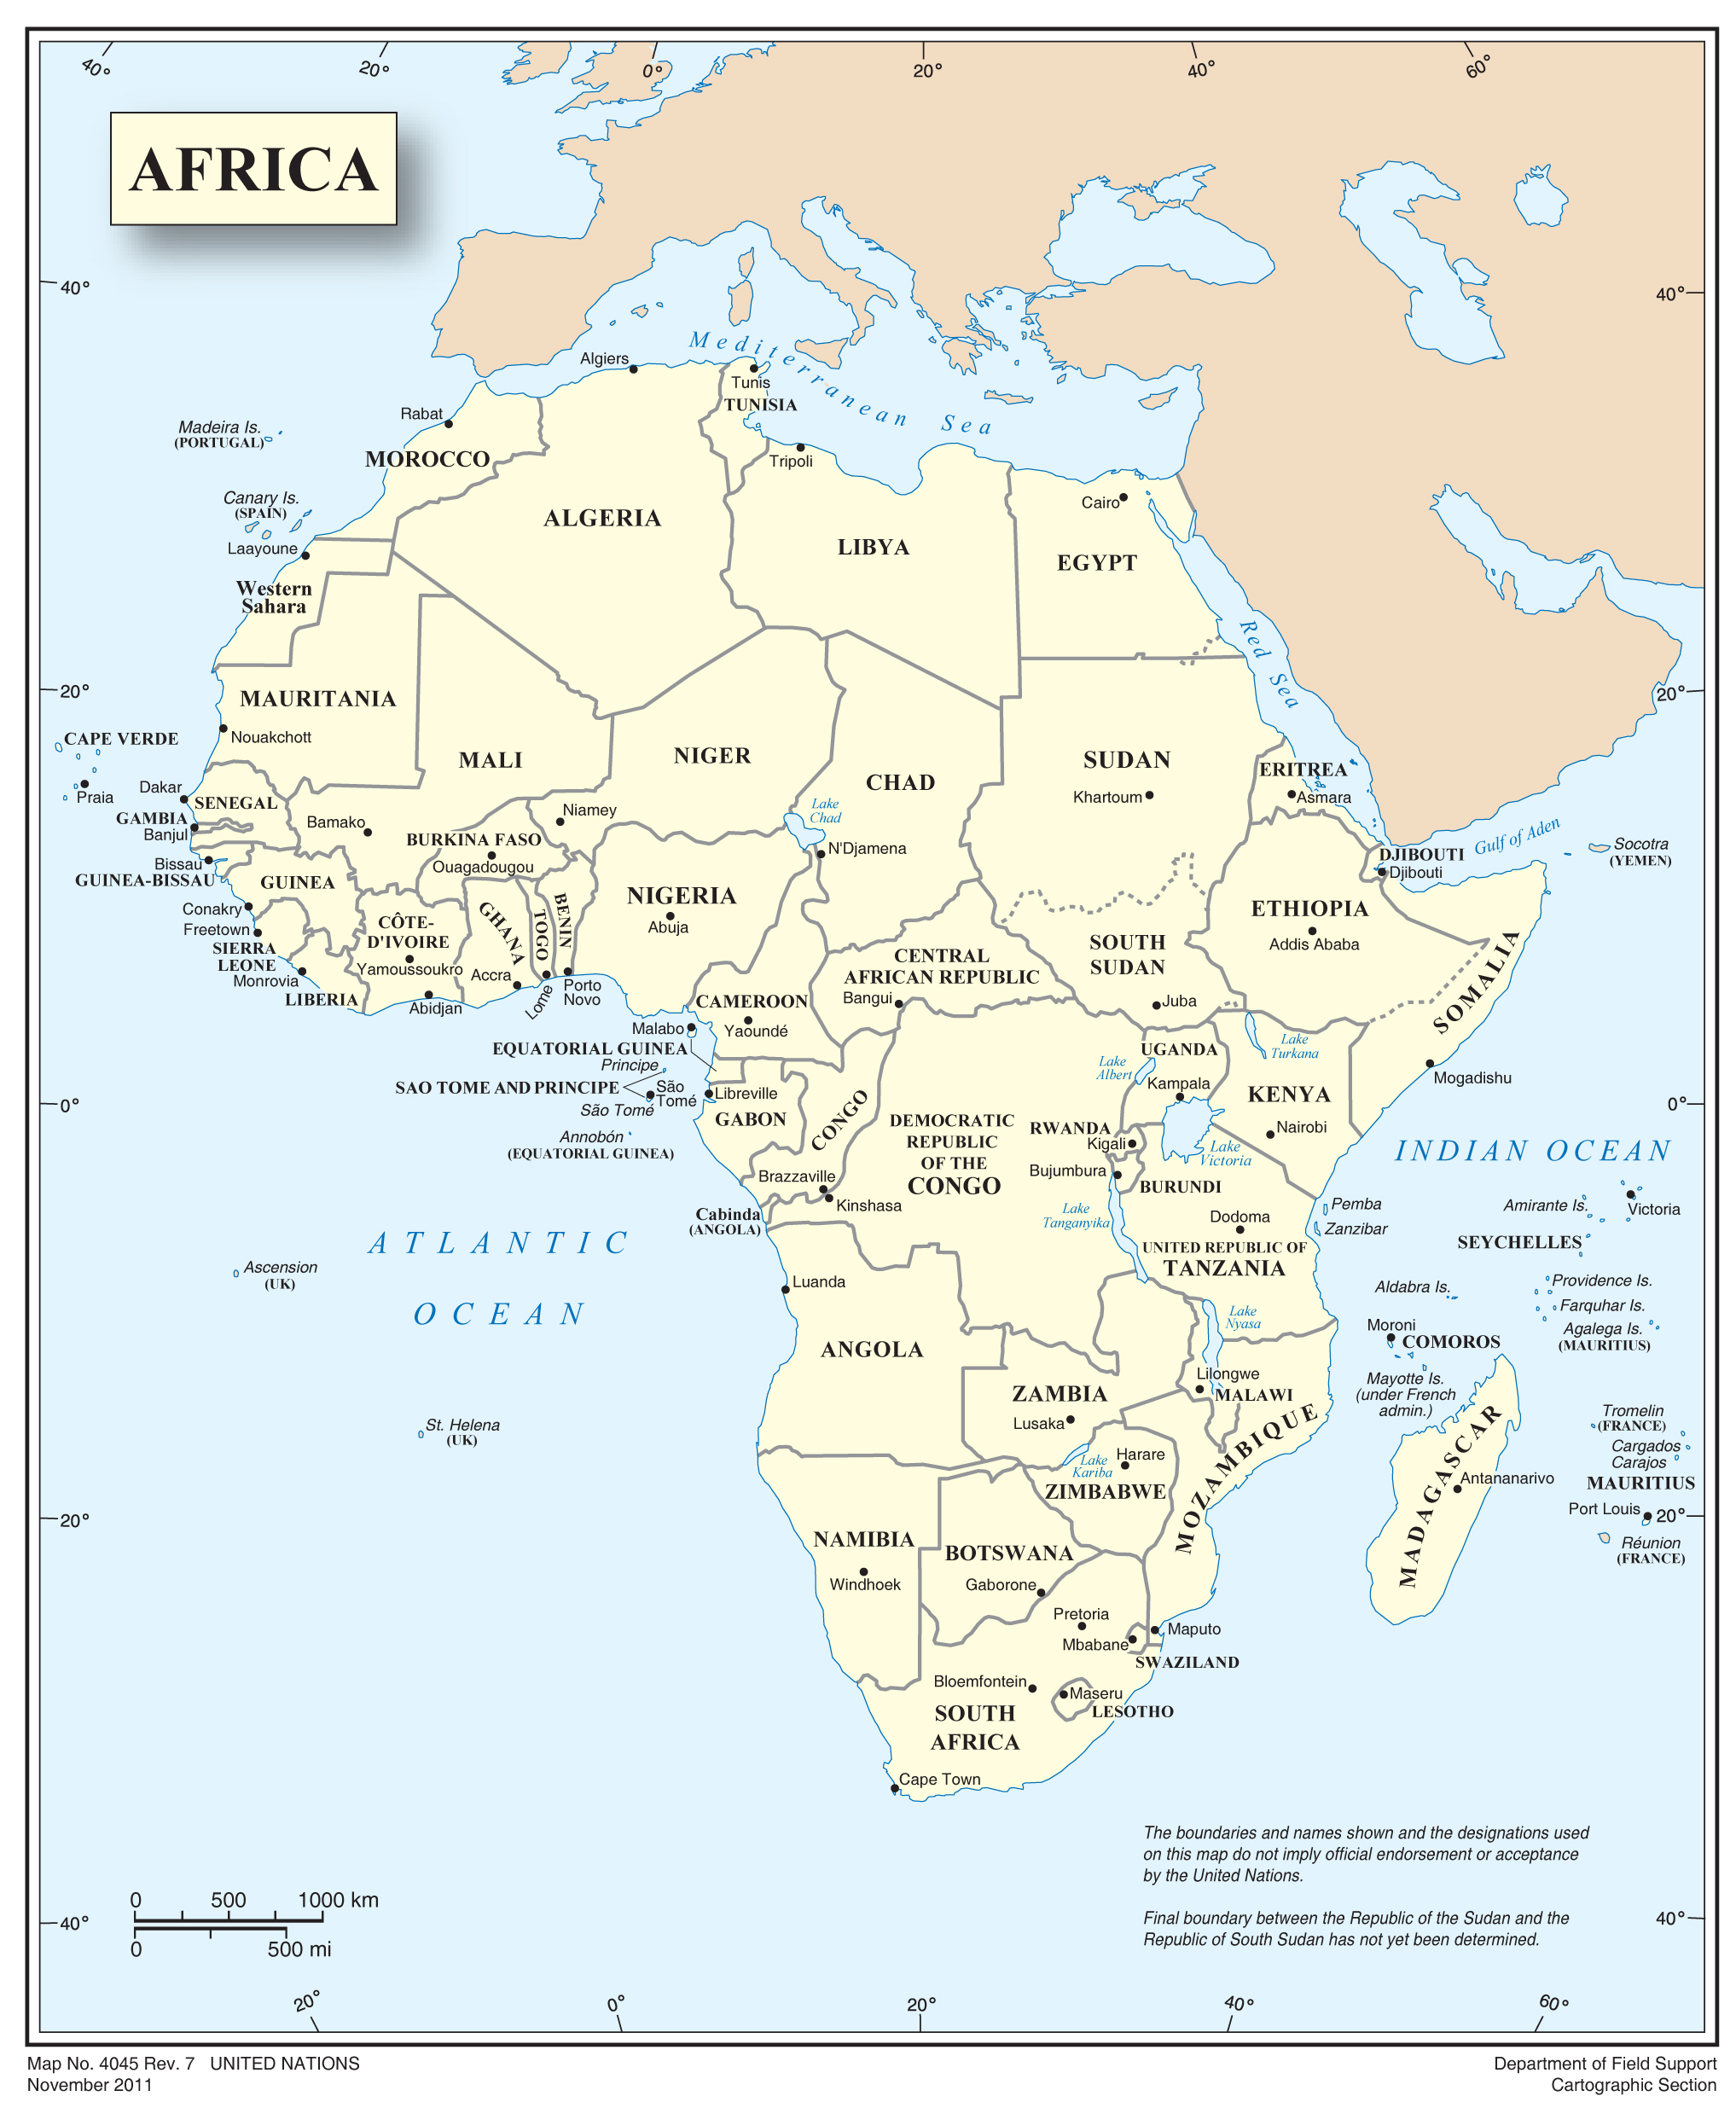
\includegraphics[width=\linewidth]{figs/africa.jpg}\\
	 	\texttt{africa.jpg}
	\end{columns}
		\vspace{-0.2cm}
	\centering \tiny{\href{http://www.pythonforbeginners.com/gui/how-to-use-pillow}{(Source)}}
\end{frame}

\subsection{Example 3: List a directory contents}
\begin{frame}{Cool code examples}{Example 3: List a directory contents}
		\vspace{-0.2cm}
		\begin{block}{dir.py}
		\vspace{-0.2cm}
		\lstinputlisting{code/dir.py}
		\vspace{-0.2cm}
		\end{block}

		\vspace{-0.2cm}
	\centering \tiny{\href{http://www.pythonforbeginners.com/code-snippets-source-code/having-fun-with-os-walk-in-python/}{(Source)}}
\end{frame}

\subsection{Example 4: Send an email with Gmail}
\begin{frame}{Cool code examples}{Example 4: Send an email with Gmail}
	\begin{columns}
 	   \column{1.1\textwidth}
		\vspace{-0.2cm}
		\begin{block}{gmail.py}
		\vspace{-0.2cm}
		\lstinputlisting{code/gmail.py}
		\end{block}
	\end{columns}

	\centering \tiny{\href{http://www.pythonforbeginners.com/code-snippets-source-code/using-python-to-send-email/}{(Source)}}
\end{frame}

\appendix
\section<Bibliographic references>*{\appendixname}
\subsection<Bibliographic references>*{Bibliographic references}

\begin{frame}[plain,allowframebreaks]
  \frametitle<presentation>{Bibliographic references}

  \begin{thebibliography}{2}
  
  \beamertemplatebookbibitems
  % libro
   \bibitem{vanRosum}[van Rosum, 2012]
    G. van Rossum, Jr. Fred L. Drake.
    \newblock \emph{Python Tutorial Release 3.2.3, chapter 6}.
    \newblock Python Software Foundation, 2012. 
  % libro
   \bibitem{Lutz}[Lutz, 2013]
    M. Lutz.
    \newblock \emph{Learning Python}.
    \newblock O'Reilly, 2013.
    
     \bibitem{Bahit}[Bahit, 2008]
     E. Bahit.
    \newblock \emph{Curso: Python para principiantes}.
    \newblock Creative Commons Atribución-NoComercial 3.0, 2012.
 \newpage
    
    \bibitem{vanRosum}[vanRosum, 2012]
    G. van Rossum, Jr. Fred L. Drake.
    \newblock \emph{The Python Library Reference. Release 3.2.3}.
    \newblock Python Software Foundation, 2012. 
    
    \bibitem{Hellman}[Hellman, 2011]
     D. Hellman.
    \newblock \emph{The Python Standard Library by Example (Developer's Library)}.
    \newblock Addison Wesley Professional, 2011.
    
    % \bibitem{Swaroop}[Swaroop, 2008]
   %  C. H. Swaroop.
   % \newblock \emph{A byte of Python}.
   % \newblock Creative Commons Atribucion-NoComercial 3.0, 2008.
 

 
  \end{thebibliography}

\end{frame}



\end{document}
